% Chapter 3
\chapter{بررسی اختصاصی پیشینه روش‌های حل مشکل ناهمگنی آماری}

\section{مقدمه}
یکی از چالش‌های اصلی در یادگیری فدرال، مسئله داده‌های غیرمستقل و غیریکنواخت
\lr{(non-IID)} 
است که منجر به بروز مشکلات آماری و تفاوت‌های داده‌ای می‌شود. این موضوع می‌تواند باعث کاهش کارایی مدل‌های یادگیری در استفاده از داده‌های توزیع‌شده شود. به دلیل اهمیت این مسئله، بسیاری از پژوهشگران تلاش‌های زیادی برای رفع این مشکل انجام داده‌اند.

مبحث اصلی این پایان‌نامه نیز به طور دقیق به همین مسئله اشاره دارد و به دنبال یافتن راه‌حلی مؤثر برای مقابله با داده‌های
\lr{non-IID}
است. در ادامه، به صورت خلاصه به بررسی راه‌حل‌هایی که تاکنون برای حل این مشکل مطرح شده‌اند، پرداخته خواهد شد. همچنین باید توجه داشت که هر یک از این راه‌حل‌ها نقاط قوت و ضعف خاص خود را دارند و بسته به شرایط و نوع داده‌ها، می‌توانند نتایج متفاوتی را به همراه داشته باشند. بررسی دقیق این راه‌حل‌ها و ارزیابی کارایی آن‌ها می‌تواند به بهبود سیستم‌های یادگیری فدرال و غلبه بر مشکلات مرتبط با داده‌های غیرمستقل و غیر یکنواخت کمک شایانی کند.

\section{نگرش برپایه داده}
\subsection{اشتراک‌گذاری داده}
مشکل اصلی الگوریتم
\lr{FedAvg}
در مواجهه با داده‌های غیرمستقل و غیریکنواخت، تفاوت وزن‌های اولیه در شروع فرآیند آموزش است. این تفاوت‌ها می‌توانند باعث شوند که مدل‌های محلی در هر گره به طور قابل توجهی متفاوت از یکدیگر باشند، که در نتیجه منجر به مشکلات همگرایی و کاهش کارایی مدل نهایی می‌شود.

برای رفع این مشکل، روشی
بر پایه اشتراک‌گذاری داده در
\cite{zhao2018federated}
پیشنهاد شده است که در آن ابتدا سرور مرکزی مقدار کمی از داده‌ها را به صورت محلی آموزش می‌دهد. در این مرحله، سرور مرکزی با استفاده از این داده‌ها، یک مدل اولیه را آموزش داده و وزن‌های اولیه آن را تنظیم می‌کند. سپس، این وزن‌های اولیه به همراه داده‌های آموزش دیده شده به تمامی کاربران ارسال می‌شود. این اقدام باعث می‌شود که تمام کاربران در ابتدای فرآیند آموزش با مجموعه‌ای از داده‌های مشترک و وزن‌های اولیه مشابه روبه‌رو شوند.

نقطه قوت این روش در این است که به دلیل انجام این عملیات تنها در آغاز فرآیند آموزش، هزینه زیادی به شبکه تحمیل نمی‌شود. در واقع، انتقال داده‌ها و وزن‌ها فقط در ابتدا انجام شده و پس از آن کاربران به صورت مستقل به آموزش مدل‌های محلی خود ادامه می‌دهند. این اقدام منجر به کاهش اختلافات ناشی از ناهمگنی داده‌ها شده و فرآیند همگرایی مدل نهایی سریع‌تر و با دقت بیشتری انجام می‌شود.

در شکل
\ref{share_data}%
، نحوه اجرای این روش و مراحل مختلف آن به تصویر کشیده شده است. این تصویر نشان می‌دهد که چگونه سرور مرکزی ابتدا داده‌های کمی را آموزش می‌دهد، وزن‌های اولیه را تنظیم می‌کند و سپس این وزن‌ها و داده‌ها را به کاربران ارسال می‌کند تا فرآیند آموزش محلی با یک نقطه شروع مشترک برای همه کاربران آغاز شود.


\begin{figure}[t]
	\centering
	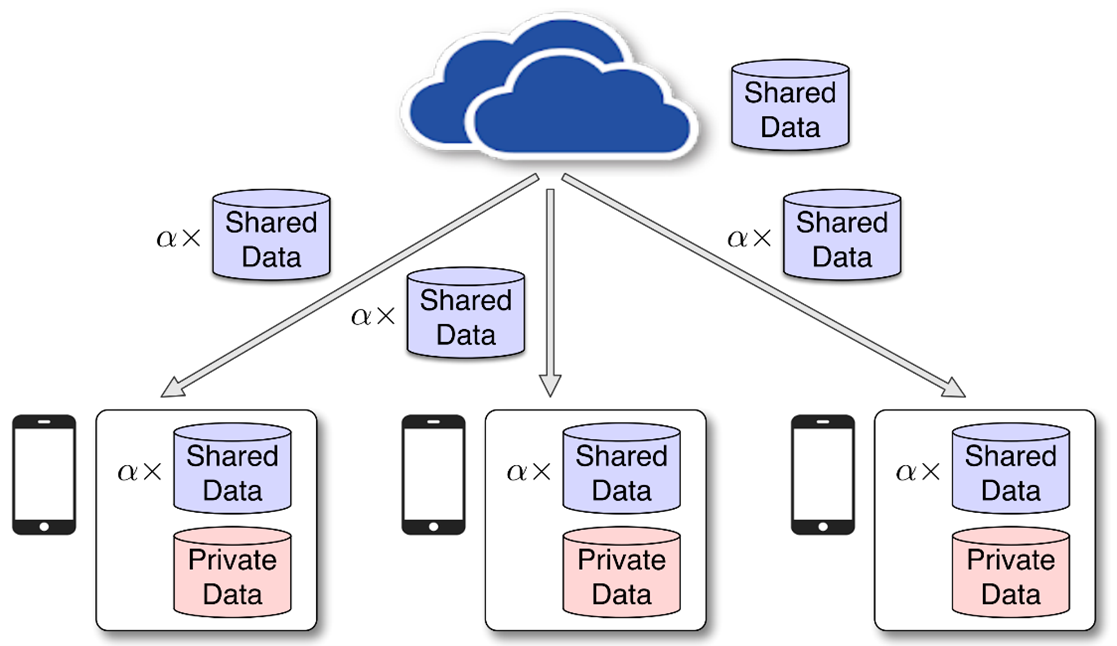
\includegraphics[scale=0.9]{images/chap3/share_data.png}%
	\caption{%
		نمایش نحوه به اشتراک‌ گذاری داده
		\cite{zhao2018federated}%
		.
	}
	\label{share_data}
	\centering
\end{figure}


یکی دیگر از روش‌های مطرح شده در زمینه یادگیری فدرال به این صورت است که کاربران بتوانند نتایج آموزش تعدادی داده اشتراکی را با یکدیگر به اشتراک بگذارند و از نتایج دیگر کاربران بر روی این داده‌های اشتراکی مطلع شوند. در این روش، کاربران نتایج به‌دست آمده از آموزش داده‌های مشترک را با هم مبادله می‌کنند، که این کار منجر به بهبود عملکرد مدل‌های محلی و در نهایت مدل سراسری می‌شود
\cite{collins2021exploiting}.

براساس بررسی‌های انجام شده، برای مثال در مجموعه داده‌ای تنها با 60٬000 داده ورودی، اگر حدود 5 درصد از داده‌ها به صورت اشتراکی در اختیار کاربران قرار گیرد، دقت مدل تا حدود 30 درصد افزایش خواهد یافت. این افزایش دقت به دلیل همگرایی بهتر مدل‌ها و کاهش تفاوت‌های آماری بین داده‌های محلی است. به عبارتی دیگر، این روش کمک می‌کند که مدل‌ها با یکدیگر هماهنگ‌تر شوند و نتایج دقیق‌تری ارائه دهند.

با این حال، باید توجه داشت که اشتراک‌گذاری داده‌ها بین کاربران می‌تواند مسائل حریم شخصی را به همراه داشته باشد. به عبارت دیگر، هنگامی که داده‌های اشتراکی بین کاربران مبادله می‌شود، احتمال نقض حریم شخصی کاربران افزایش می‌یابد. بنابراین، هنگام پیاده‌سازی این روش، ضروری است که اقدامات لازم برای حفظ حریم شخصی کاربران به طور جدی مد نظر قرار گیرد. این اقدامات می‌تواند شامل استفاده از تکنیک‌های رمزنگاری، ناشناس‌سازی داده‌ها، یا روش‌های دیگر برای محافظت از اطلاعات حساس کاربران باشد
\cite{ma2022state}.

در نهایت، روش به اشتراک‌گذاری داده‌ها بین کاربران، اگرچه می‌تواند به بهبود دقت و کارایی مدل‌ها کمک کند، اما نیازمند دقت و توجه ویژه‌ای به مسائل حریم شخصی است. پژوهشگران و توسعه‌دهندگان باید با در نظر گرفتن این چالش‌ها، راهکارهایی را برای حفظ امنیت و حریم شخصی کاربران در هنگام اجرای این روش‌ها ارائه دهند.

\subsection{
	بهبود داده%
\LTRfootnote{Data Enhancement}
}
ابتدا، کاربران تعدادی از داده‌های خود را به سمت سرور ارسال می‌کنند. سرور، با استفاده از داده‌های دریافتی، یک مدل شبکه مولد رقابتی%
\LTRfootnote{Generative Adversarial Network (GAN)}
ایجاد می‌کند و این مدل را برای تمامی کاربران ارسال می‌نماید. کاربران با استفاده از این شبکه مولد رقابتی و با توجه به داده‌های خود، تعدادی داده جدید تولید کرده و در مراحل بعدی آموزش از این داده‌ها نیز استفاده می‌کنند. به این ترتیب، شبکه مولد رقابتی به کاربران کمک می‌کند تا داده‌های بیشتری برای آموزش مدل‌های خود در اختیار داشته باشند و از این داده‌ها برای بهبود عملکرد مدل‌های خود استفاده کنند. در شکل
\ref{gan}
نحوه عملکرد این روش به تصویر کشیده شده است.

این روش، به دلیل استفاده از تکنیک‌های رمزگذاری%
\LTRfootnote{Encoding}
و رمزگشایی%
\LTRfootnote{Decoding}
داده‌ها، نسبت به روش‌های اشتراک‌گذاری داده‌ها از نظر حفظ حریم شخصی کاربران بهتر عمل می‌کند. به این معنی که، به جای ارسال داده‌های خام کاربران به سرور یا دیگر کاربران، از داده‌های تولید شده توسط شبکه مولد رقابتی استفاده می‌شود که احتمال نقض حریم شخصی را کاهش می‌دهد.
به عبارت دیگر، حتی اگر داده‌ها در طول انتقال یا در سرور مورد دسترسی غیرمجاز قرار گیرند، به دلیل رمزگذاری، اطلاعات واقعی کاربران فاش نخواهد شد. این ویژگی، امنیت و حریم شخصی کاربران را به طور قابل توجهی افزایش می‌دهد و از اطلاعات حساس آنان در برابر تهدیدات محافظت می‌کند
\cite{jeong2018communication}.

بنابراین، روش‌های بهبود داده که مبتنی بر رمزگذاری و رمزگشایی داده‌ها هستند،
در حالی که تلاش می‌کنند عملکرد مدل‌های یادگیری را بهبود بخشند،
از حریم شخصی کاربران نیز حفاظت می‌نمایند. این ترکیب از امنیت و کارایی، این روش‌ها را به گزینه‌های مناسبی برای استفاده در سیستم‌های یادگیری فدرال تبدیل کرده است.

\begin{figure}[t]
	\centering
	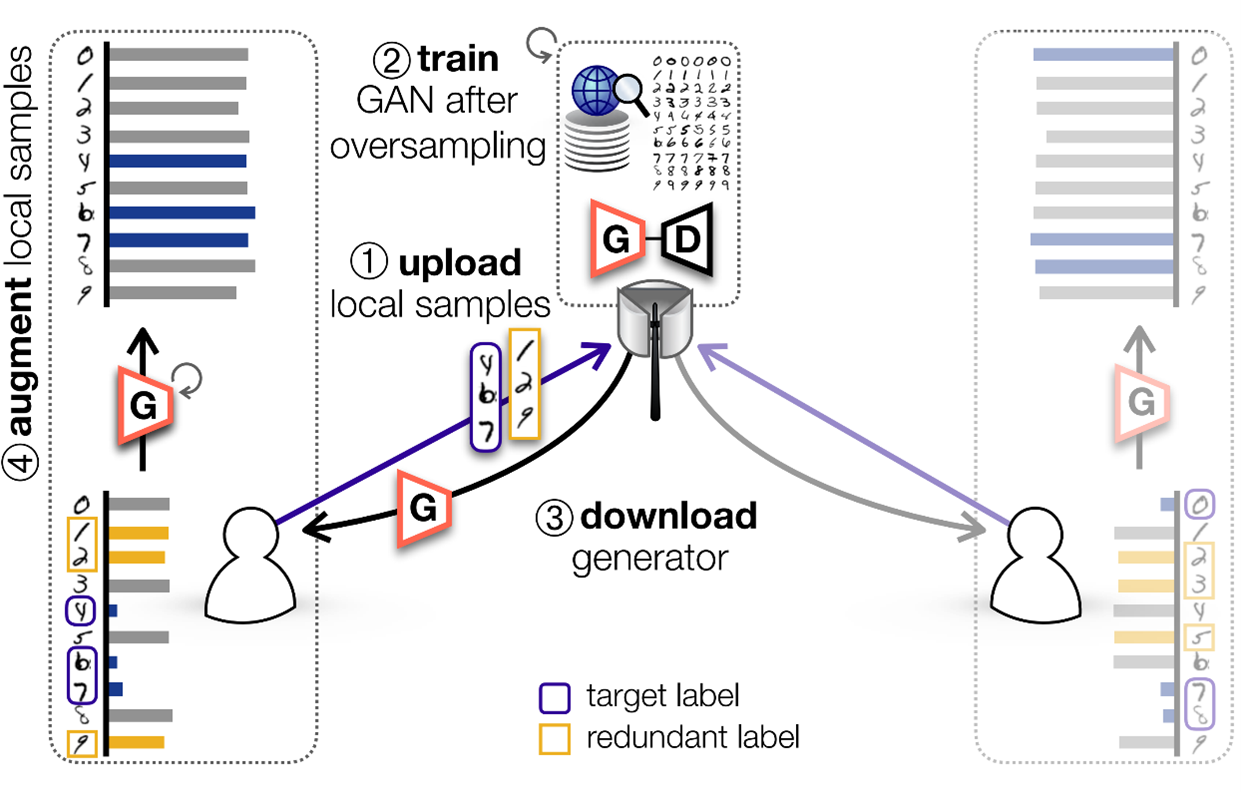
\includegraphics[scale=0.9]{images/chap3/generative_adversarial_network.png}%
	\caption{%
		استفاده از شبکه مولد رقابتی جهت تولید داده
		\cite{jeong2018communication}%
		.
	}
	\label{gan}
	\centering
\end{figure}

\subsection{انتخاب داده}
در هنگام انتخاب کاربران برای فرآیند آموزش، می‌توان از الگوریتم‌هایی که بر پایه کیفیت داده‌ها عمل می‌کنند، استفاده نمود. به عبارت دیگر، می‌توان از الگوریتم حریصانه کوله‌پشتی برای اولویت‌بندی کاربران بهره برد، به نحوی که کاربران با داده‌های غنی و گسترده‌تر، اولویت بالاتری جهت انتخاب داشته باشند. این رویکرد به بهبود کیفیت آموزش کمک می‌کند، زیرا داده‌های با کیفیت بالاتر تاثیر مثبتی بر نتایج نهایی مدل خواهند داشت
\cite{taik2021data}.

علاوه بر این، می‌توان از روش‌های یادگیری عمیق برای تخمین زمان اجرای مدل در سمت کاربران استفاده کرد. این روش‌ها می‌توانند زمان مورد نیاز برای اجرای مدل را پیش‌بینی کنند و بر اساس این پیش‌بینی، از بین ویژگی‌های مختلف جهت آموزش، تنها آن‌هایی را انتخاب نمایند که تاثیر بیشتری بر خروجی خواهند داشت. به این ترتیب، با بهینه‌سازی انتخاب ویژگی‌ها، می‌توان زمان و منابع محاسباتی را به شکل موثرتری مدیریت کرد.

یکی از نکات کلیدی در استفاده از این روش‌های انتخاب داده این است که هیچ کدام از آن‌ها تغییری بر روی داده‌ها و کاربران ایجاد نمی‌کنند. به عبارت دیگر، این روش‌ها به گونه‌ای طراحی شده‌اند که داده‌های موجود و وضعیت کاربران بدون تغییر باقی می‌مانند، اما فرآیند انتخاب و استفاده از داده‌ها بهینه‌تر و کارآمدتر می‌شود. این ویژگی، استفاده از این راه‌حل‌ها را در برنامه‌های مختلف بسیار کاربردی و موثر می‌سازد
\cite{zeng2022local}.

در نتیجه، استفاده از الگوریتم‌های مبتنی بر کیفیت داده‌ها و روش‌های یادگیری عمیق برای تخمین زمان اجرا، می‌تواند به طور قابل توجهی فرآیند آموزش در سیستم‌های یادگیری فدرال را بهبود بخشد. این روش‌ها نه تنها کیفیت داده‌های مورد استفاده را افزایش می‌دهند، بلکه با بهینه‌سازی منابع محاسباتی و زمان اجرا، کارایی سیستم را نیز بهبود می‌بخشند. این ترکیب از بهینه‌سازی داده‌ها و مدیریت منابع، به ویژه در محیط‌های با منابع محدود، اهمیت ویژه‌ای دارد و می‌تواند به نتایج بهتری در آموزش مدل‌ها منجر شود.


\section{نگرش برپایه مدل}
\subsection{
	تجمیع و به‌روزرسانی مدل%
\LTRfootnote{Model Update and Aggregation}
}	
هنگام اجرای الگوریتم در مراحل میانی، می‌توان با استفاده از ساختار شبکه‌های عصبی عمیق موجود، تفاوت گره‌های شبکه بین کاربران مختلف را بررسی نمود. این بررسی به ما امکان می‌دهد تا ساختار مدل اصلی را بر اساس تفاوت‌ها و ویژگی‌های مختلف کاربران، بهبود بخشیم و در نتیجه مدل کارآمدتری ایجاد کنیم. این فرآیند می‌تواند به بهینه‌سازی عملکرد مدل و افزایش دقت آن در مراحل بعدی کمک کند
\cite{sannara2021federated}.

روش دیگری برای بهبود عملکرد یادگیری فدرال این است که هم در سمت سرور و هم در سمت کاربران چندین مدل شبکه عصبی قرار داده شود. این شبکه‌ها به صورت جداگانه آموزش داده شده و به‌روزرسانی می‌شوند. پس از چند مرحله آموزش، می‌توان با استفاده از الگوریتم‌های تطابق بهترین، شبکه‌ها را با یکدیگر ترکیب کرد. این رویکرد به بهبود عملکرد کلی مدل کمک می‌کند و باعث می‌شود تا مدل نهایی از ویژگی‌ها و مزایای چندین شبکه عصبی بهره‌مند شود
\cite{qin2021mlmg}.
در شکل
\ref{multi_local_and_multi_global}
نحوه عملکرد این روش به تصویر کشیده شده است. 

همچنین، مکانیزم یادگیری فدرال نیمه-ناهمزمان%
\LTRfootnote{Semi-Asynchronous}
نیز یکی دیگر از روش‌های موثر در این حوزه است. در این روش، مدل‌های کاربران به ترتیبی که به سرور می‌رسند به‌روزرسانی می‌شوند. این رویکرد به خوبی با کاربران کند%
\LTRfootnote{Stragglers}
که ممکن است در گردش‌های مختلف به سرور بپیوندند، سازگار است. با به‌روزرسانی و ترکیب مدل‌ها در مراحل مختلف، این مکانیزم به خوبی می‌تواند توازن را برای داده‌های ناهمگن برقرار کند و عملکرد مدل را بهینه سازد
\cite{ma2021fedsa, ma2022state}.

در نهایت، با استفاده از این رویکردها و الگوریتم‌ها می‌توان به طور موثرتری با چالش‌های موجود در یادگیری فدرال مقابله کرد و مدل‌هایی با دقت و کارایی بالاتر ایجاد نمود. این روش‌ها نه تنها به بهبود ساختار مدل‌ها کمک می‌کنند، بلکه باعث می‌شوند تا فرآیند آموزش بهینه‌تر و سازگارتر با تنوع و ناهمگنی داده‌ها انجام شود.


\subsection{
	بهینه‌سازی تطبیقی%
\LTRfootnote{Adaptive Optimization}
}
الگوریتم پیش‌بینی میزان‌کار به گونه‌ای طراحی شده است که به صورت خودکار اطلاعات جامعی از سابقه آموزش هر کاربر را جمع‌آوری می‌کند. این اطلاعات شامل عملکرد کاربر در مراحل قبلی آموزش است. سپس بر اساس این سوابق، میزان پیچیدگی الگوریتم برای مرحله بعدی آموزش تعیین می‌شود تا برای کاربر مربوطه مناسب باشد . این رویکرد به بهینه‌سازی فرآیند آموزش کمک می‌کند و موجب می‌شود تا الگوریتم‌ها به شکل موثرتری با توانایی‌های هر کاربر هماهنگ شوند
\cite{li2021fedsae}.

یکی از روش‌های اولیه در بهینه‌سازی تطبیقی، استفاده از روش کاهش نرخ یادگیری است. در این روش، نرخ یادگیری برای هر کاربر به طور جداگانه و بر اساس عملکرد گذشته وی تعیین می‌شود. این به معنای آن است که کاربران با عملکرد بهتر ممکن است نرخ یادگیری بالاتری داشته باشند، در حالی که برای کاربرانی که با مشکلاتی مواجه بوده‌اند، این نرخ کاهش می‌یابد تا فرآیند یادگیری بهبود یابد
\cite{reddi2020adaptive}.

در طول سال‌های اخیر، بهینه‌سازی تطبیقی نشان داده است که می‌تواند تاثیر قابل‌توجهی بر بهبود عملکرد الگوریتم‌ها داشته باشد. به همین دلیل، محققان به سمت توسعه روش‌هایی رفته‌اند که امکان تغییر و تطبیق پارامترهای الگوریتم را در طول زمان فراهم کنند. این رویکرد باعث می‌شود تا هر کاربر بتواند در مراحل مختلف آموزش، پارامترهای مربوط به الگوریتم را متناسب با نیازها و شرایط خود تنظیم کند. این انعطاف‌پذیری به الگوریتم‌ها کمک می‌کند تا با گذشت زمان کارایی بیشتری داشته باشند و به طور خاص‌تر با شرایط و نیازهای کاربران سازگار شوند.

به طور کلی، استفاده از الگوریتم‌های پیش‌بینی و بهینه‌سازی تطبیقی می‌تواند به شکل چشم‌گیری کیفیت آموزش و کارایی سیستم‌های یادگیری را بهبود بخشد. این روش‌ها با فراهم کردن امکان تنظیم پارامترهای آموزشی بر اساس سوابق و عملکرد کاربران، موجب می‌شوند تا فرآیند یادگیری به شکل دقیق‌تر و موثرتری انجام شود. در نتیجه، کاربران می‌توانند از تجربیات گذشته خود بهره ببرند و با شرایط بهتر و مناسبتری به یادگیری ادامه دهند.


\begin{figure}[t]
	\centering
	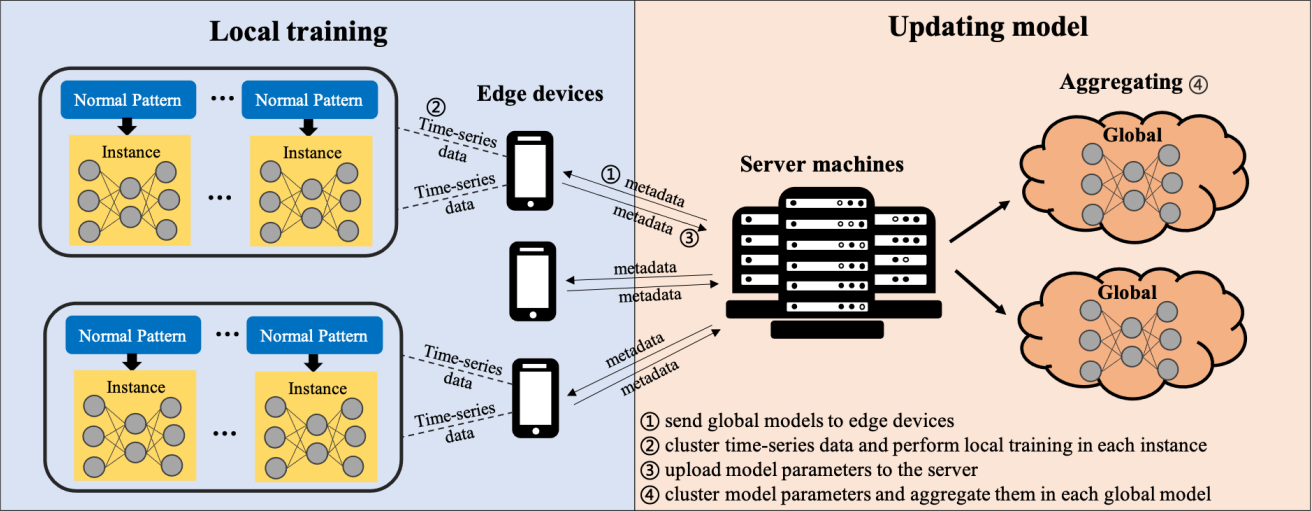
\includegraphics[scale=0.44]{images/chap3/multi_local_and_multi_global.png}%
	\caption{%
		چارچوب یک سیستم یادگیری فدرال چندمحلی و چندمرکزی برای کشف ناهنجاری‌ها 
		\cite{qin2021mlmg}%
		.
	}
	\label{multi_local_and_multi_global}
	\centering
\end{figure}


\subsection{بهینه‌سازی منظم}
از مهم‌ترین و پرکاربردترین روش‌های موجود جهت کنترل داده‌های غیرمستقل و غیریکنواخت، رویکردهای بهینه‌سازی منظم هستند. این رویکردها با هدف بهبود فرآیند یادگیری و کاهش نوسانات ناشی از تفاوت در توزیع داده‌ها به کار گرفته می‌شوند. به عنوان مثال، یکی از روش‌های متداول در این زمینه، در نظر گرفتن نزدیک‌ترین همسایه است که طی آن تابع بهینه‌سازی محلی برای هر کاربر به‌روزرسانی می‌شود تا از نوسانات زیاد جلوگیری کند و هماهنگی بیشتری بین داده‌های مختلف کاربران ایجاد شود
\cite{li2020federatedheteroneneous}.

یکی دیگر از روش‌های معروف در این زمینه، مکانیزم استاد-دانشجو%
\LTRfootnote{Teacher-Student}
است. در این روش، یک مدل به عنوان استاد و مدل‌های دیگر به عنوان دانشجو عمل می‌کنند. گرادیان‌ها برای هر کاربر توسط یک جمله اضافه شده به نام جمله منظم‌سازی%
\LTRfootnote{Regularization Term}
تنظیم می‌شود. این جمله منظم‌سازی به منظور کاهش خطاها و بهبود دقت مدل‌ها افزوده می‌شود و از بیش‌برازش%
\LTRfootnote{Overfitting}
جلوگیری می‌کند
\cite{li2020communication}.

رویکردهای بهینه‌سازی منظم، همان‌طور که در حوزه‌های مختلف یادگیری ماشین و یادگیری عمیق توانسته‌اند کارایی خود را به اثبات برسانند، در یادگیری فدرال نیز عملکرد بسیار خوبی دارند. این رویکردها با تنظیم مدل‌ها به گونه‌ای که نوسانات ناشی از داده‌های مختلف را کاهش دهند، به بهبود عملکرد کلی سیستم کمک می‌کنند. همچنین، با جلوگیری از بیش‌برازش، مدل‌ها را به سمت تعمیم بهتر هدایت می‌کنند، که این امر در محیط‌هایی با داده‌های غیرمستقل و غیریکنواخت بسیار حیاتی است.

در مجموع، استفاده از روش‌های بهینه‌سازی منظم در یادگیری فدرال نه تنها باعث بهبود دقت مدل‌ها می‌شود، بلکه موجب می‌گردد تا فرآیند یادگیری با پایداری و کارایی بیشتری انجام شود. این رویکردها به دلیل توانایی‌شان در کنترل نوسانات و کاهش خطاها، از ابزارهای اساسی در یادگیری فدرال به شمار می‌آیند و به توسعه مدل‌های دقیق و قابل اعتماد کمک می‌کنند.



\section{نگرش برپایه چهارچوب}
\subsection{
	خوشه‌بندی مشابهت%
\LTRfootnote{Similarity Clustering}
}
خوشه‌بندی یکی از روش‌های بسیار پرکاربرد و مهم در حوزه یادگیری ماشین است که ایده‌های آن می‌توانند در یادگیری فدرال نیز مورد استفاده قرار گیرند. در این روش، هنگامی که کاربران مدل‌های خود را آموزش داده و به سرور ارسال می‌کنند، سرور بر اساس مدل‌های دریافتی شباهت‌های آن‌ها را بررسی کرده و کاربرانی که مدل‌های مشابه دارند را در یک خوشه قرار می‌دهد. این فرایند به سرور امکان می‌دهد تا در مراحل بعدی، مدل یکسانی را برای اعضای هر خوشه ارسال کند. این رویکرد باعث می‌شود که مدل‌های آموزش‌دیده شده توسط کاربران با داده‌های مشابه، به طور همزمان و هماهنگ بهبود یابند و از همگرایی بهتری برخوردار شوند
\cite{ghosh2019robust}.

به طور معمول، پس از چندین دوره آموزشی، فرآیند خوشه‌بندی مجدداً تکرار می‌شود تا از به‌روزرسانی‌های جدید و تغییرات احتمالی در داده‌ها و مدل‌ها بهره‌برداری شود. در شکل
\ref{similarity_clustering}%
، حالت کلی خوشه‌بندی شباهت در سیستم‌های فدرال به تصویر کشیده شده است.

با وجود تمام مزایایی که روش خوشه‌بندی مشابهت به همراه دارد، یکی از مهم‌ترین مشکلات آن هزینه بالای ارتباطات است. در این روش، نیاز است که ساختار خوشه‌بندی در مراحل مختلف ارسال و دریافت شود، که این فرایند می‌تواند هزینه زیادی را بر شبکه اعمال کند. به خصوص در محیط‌هایی با تعداد زیاد کاربران و داده‌های بزرگ، این هزینه‌ها به طور قابل توجهی افزایش می‌یابد و می‌تواند عملکرد کلی سیستم را تحت تأثیر قرار دهد.

بنابراین، در حالی که خوشه‌بندی شباهت می‌تواند کارایی و دقت یادگیری فدرال را بهبود بخشد، باید به دقت هزینه‌های ارتباطی آن نیز مورد ارزیابی قرار گیرد و در صورت امکان، بهینه‌سازی‌های لازم انجام شود تا این هزینه‌ها کاهش یابند. به کارگیری روش‌های بهینه‌سازی ارتباطات و فشرده‌سازی داده‌ها می‌تواند در این زمینه مفید باشد و به حفظ تعادل بین کارایی و هزینه‌ها کمک کند.

\begin{figure}[t]
	\centering
	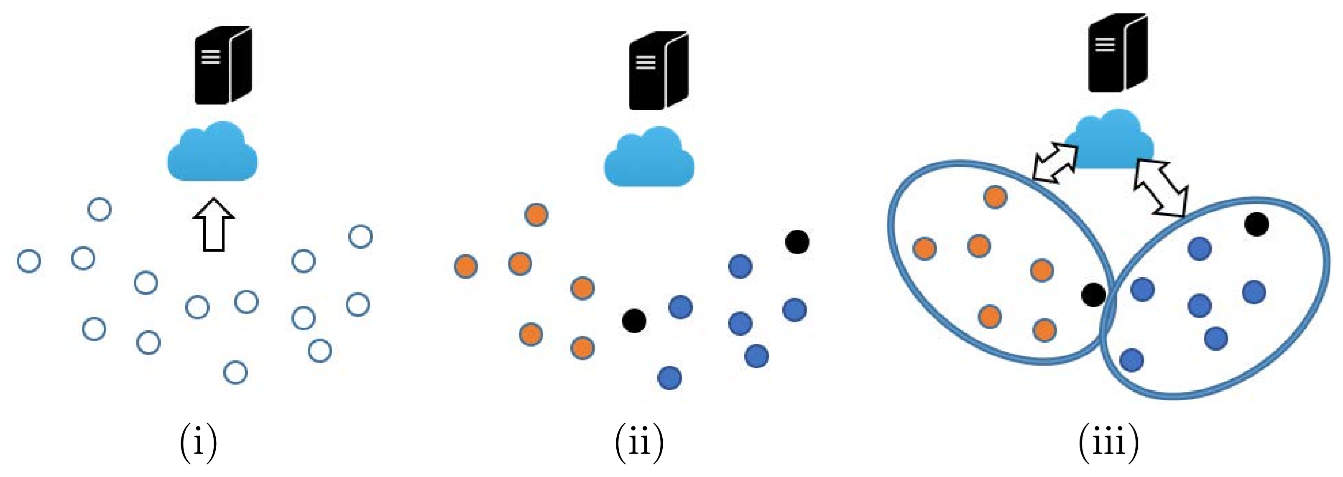
\includegraphics[scale=0.9]{images/chap3/similarity_clustering.png}%
	\caption{%
		روش خوشه‌بندی مشابهت 
		\cite{ghosh2019robust}%
		.
	}
	\label{similarity_clustering}
	\centering
\end{figure}

\subsection{
	دانش تقطیر%
\LTRfootnote{Knowledge Distillation}
}
به‌طور کلی، در روش‌های دانش تقطیر، هدف اصلی ساده‌سازی مدل‌های پیچیده و ارائه مدل‌هایی ساده اما کارآمد است. یکی از الگوریتم‌های مهم در این زمینه
\lr{DS-FL}%
\LTRfootnote{Distillation-base Semi-supervised Federated Learning}
است. این الگوریتم با استفاده از مجموعه داده‌های بدون برچسب، به جای ارسال پارامترهای مدل، تنها خروجی مدل محلی را به اشتراک می‌گذارد. این روش به‌خصوص برای داده‌های غیرمستقل و غیریکنواخت بسیار مؤثر عمل می‌کند و نتایج مطلوبی به همراه دارد.

یکی از مهم‌ترین مزایای استفاده از دانش تقطیر، کاهش چشمگیر سربار شبکه است. به دلیل اینکه در این روش به جای ارسال پارامترهای مدل‌های محلی، فقط خروجی نهایی مدل‌ها ارسال می‌شود، حجم داده‌های ارسالی به طور قابل توجهی کاهش می‌یابد. این کاهش حجم داده‌ها نه تنها هزینه‌های ارتباطی را پایین می‌آورد بلکه سرعت پردازش و به‌روزرسانی مدل‌ها را نیز افزایش می‌دهد. به این ترتیب، بهره‌وری سیستم بهبود یافته و توان محاسباتی به نحو بهتری مدیریت می‌شود.

در روش
\lr{DS-FL}%
، ابتدا هر کاربر محلی با استفاده از داده‌های خود، مدلی را آموزش می‌دهد. سپس به جای ارسال پارامترهای مدل به سرور مرکزی، تنها خروجی مدل روی داده‌های بدون برچسب به اشتراک گذاشته می‌شود. سرور مرکزی با تجمیع این خروجی‌ها، یک مدل جهانی به‌روز شده را ایجاد می‌کند و آن را برای کاربران ارسال می‌کند. این فرایند تکرار می‌شود تا مدل جهانی به بهینه‌ترین حالت ممکن برسد
\cite{itahara2021distillation}.

به کارگیری دانش تقطیر در یادگیری فدرال نه تنها به بهبود کارایی شبکه کمک می‌کند، بلکه امنیت و حریم خصوصی داده‌ها را نیز افزایش می‌دهد. چون خروجی مدل‌ها اغلب اطلاعات حساس کمتری نسبت به پارامترهای مدل در خود دارند، احتمال افشای اطلاعات شخصی کاربران کاهش می‌یابد. این ویژگی به‌خصوص در محیط‌هایی که حفظ حریم خصوصی کاربران اولویت بالایی دارد، از اهمیت ویژه‌ای برخوردار است.

به‌طور خلاصه، روش‌های دانش تقطیر مانند
\lr{DS-FL}
با هدف ساده‌سازی مدل‌های پیچیده و کاهش هزینه‌های ارتباطی، به بهبود کارایی و امنیت در سیستم‌های یادگیری فدرال کمک می‌کنند. این روش‌ها با ارسال خروجی‌های مدل به جای پارامترها، سربار شبکه را کاهش داده و به تطبیق بهتر مدل‌ها با داده‌های غیرمستقل و غیریکنواخت کمک می‌کنند.


\subsection{
	لایه‌های شخصی‌سازی%
\LTRfootnote{Personalization Layers}
}
روش لایه‌های شخصی‌سازی شده به این شکل عمل می‌کنند که در ابتدا کاربران بر اساس معیارهایی مانند کارایی آموزش و سرعت اجرا به گروه‌های مختلفی تقسیم می‌شوند. سپس، این کاربران بر اساس معیارهای تعیین شده به صورت لایه‌ای مرتب می‌شوند. به این ترتیب، سرور هنگامی که مدل را به‌روزرسانی می‌کند و قصد دارد آن را در مرحله بعد به سمت کاربران ارسال نماید، سعی می‌کند کاربرانی را که در یک لایه مشترک حضور دارند انتخاب کند. این انتخاب به سرور امکان می‌دهد تا گردش به‌روزرسانی‌ها را با سرعت و کارایی هماهنگ‌تری به پایان برساند و عملکرد بهتری از سیستم بگیرد
\cite{chai2020tifl}.

یکی از نکات کلیدی در اجرای این روش، تعیین میزان حد و آستانه‌ای است که بر اساس آن، کاربران به لایه‌های مختلف تقسیم می‌شوند. این تقسیم‌بندی باید به گونه‌ای باشد که خروجی مدل بهینه باشد و کارایی سیستم حفظ شود. تعیین این حد و آستانه‌ها می‌تواند چالش‌برانگیز باشد و نیاز به سعی و خطا دارد تا بهترین ترکیب ممکن به دست آید.

به‌طور کلی، روش لایه‌های شخصی‌سازی شده با تقسیم‌بندی کاربران و مرتب‌سازی آن‌ها در لایه‌های مختلف، امکان بهبود هماهنگی و کارایی در گردش به‌روزرسانی‌ها را فراهم می‌کند. این رویکرد نه تنها باعث می‌شود که کاربران با سرعت مشابه در یک لایه قرار گیرند، بلکه به سرور کمک می‌کند تا با کاهش ناهماهنگی‌ها، به‌روزرسانی مدل‌ها را با کارایی بیشتری انجام دهد. انتخاب صحیح معیارهای تقسیم‌بندی و آستانه‌ها در این روش، از اهمیت بالایی برخوردار است و نیازمند تحلیل و ارزیابی دقیق است تا بهترین نتایج ممکن به دست آید.




\section{نگرش برپایه الگوریتم}
\subsection{فرایادگیری}
مدل ابتدایی فرایادگیری پیاده‌شده بر بستر یادگیری فدرال، در واقع از همان الگوریتم
\lr{FedAvg}
بهره می‌برد و با ترکیب آن با روش فرایادگیری، تلاش دارد تا فرایند آموزش را بهینه‌سازی کرده و پارامترهای مناسب‌تری را به دست آورد
\cite{jiang2019improving}.
الگوریتم اولیه-دوگانه%
\LTRfootnote{Primal-Dual}
\lr{(FedPD)}%
، یکی از الگوریتم‌های کارا با استفاده از فرایادگیری است که حتی برای توابع غیرمحدب نیز مقاوم بوده و علاوه بر دستیابی به همگرایی مناسب، از نظر کاهش ارتباطات نیز بسیار کارآمد عمل می‌کند
\cite{zhang2021fedpd}.

روش‌های فرایادگیری به دلیل توانایی‌شان در هماهنگی سریع با داده‌های جدید و تغییر پارامترهای مربوطه، مورد توجه قرار گرفته‌اند. این روش‌ها می‌توانند به سرعت با شرایط جدید سازگار شوند و پارامترهای مدل را بهبود بخشند. با این حال، یکی از چالش‌های اصلی این روش‌ها مربوط به کاربران کند است. این کاربران ممکن است به دلیل محدودیت‌های سخت‌افزاری یا مشکلات ارتباطی، نتوانند به‌روزرسانی‌های سریع و هماهنگ را انجام دهند و این موضوع می‌تواند باعث اختلال در عملکرد مدل شود.

به طور کلی، مدل‌های فرایادگیری در بستر یادگیری فدرال با ترکیب روش‌های مختلف و بهره‌گیری از الگوریتم‌های بهینه‌سازی مانند
\lr{FedAvg}
و
\lr{FedPD}%
، سعی دارند تا با بهبود فرآیندهای آموزش و کاهش هزینه‌های ارتباطی، به نتایج بهتری دست یابند. این روش‌ها با وجود چالش‌هایی که ممکن است در پیاده‌سازی و هماهنگی با کاربران کند داشته باشند، به دلیل قابلیت‌هایشان در بهینه‌سازی و هماهنگی سریع با داده‌های جدید، پتانسیل بالایی برای بهبود عملکرد سیستم‌های یادگیری فدرال دارند.

\subsection{یادگیری چندوظیفه‌ای}
یادگیری چندوظیفه‌ای به این معناست که هر یک از کاربران شرکت‌کننده در فرآیند یادگیری فدرال، به دنبال یادگیری وظایف مختلفی هستند و تلاش می‌شود که در این مسیر، حریم شخصی کاربران به طور قابل‌توجهی حفظ شود. در یادگیری فدرال چندوظیفه‌ای، کاربران بر اساس داده‌های محلی خود، مدل را آموزش می‌دهند و نتایج آن را به سمت سرور مرکزی ارسال می‌کنند. سپس سرور، با تحلیل پارامترهای ارسال شده، روابط معناداری میان این مدل‌ها پیدا کرده و مدل به‌روز شده را دوباره به سمت کاربران بازمی‌گرداند
\cite{corinzia2019variational}.

به عبارت دیگر، در این روش، هر کاربر ابتدا مدل را با استفاده از داده‌های محلی خود آموزش می‌دهد. این فرآیند موجب می‌شود که داده‌های شخصی کاربران از دستگاه‌های آنان خارج نشود و فقط نتایج به دست آمده از مدل‌های محلی به سرور ارسال شود. سرور مرکزی با جمع‌آوری این نتایج، به دنبال یافتن الگوها و روابطی است که بتواند مدل کلی را بهبود بخشد. این مدل بهبود یافته سپس به کاربران ارسال می‌شود تا مجدداً با داده‌های محلی آنان آموزش داده شود.

در شکل
\ref{multi_tasking}%
، نمای کلی از نحوه عملکرد یادگیری چندوظیفه‌ای در سیستم‌های فدرال به نمایش گذاشته شده است. این شکل به خوبی نشان می‌دهد که چگونه هر کاربر با استفاده از داده‌های محلی خود مدل را آموزش داده و نتایج را به سرور ارسال می‌کند و سرور با تحلیل این نتایج، مدل بهبود یافته را به کاربران بازمی‌گرداند.

به طور کلی، یادگیری چندوظیفه‌ای فدرال، به دلیل توانایی‌اش در تطبیق با داده‌های متنوع و محافظت از حریم خصوصی کاربران، یک رویکرد بسیار مؤثر و کارآمد در زمینه یادگیری فدرال محسوب می‌شود.

\begin{figure}[b!]
	\centering
	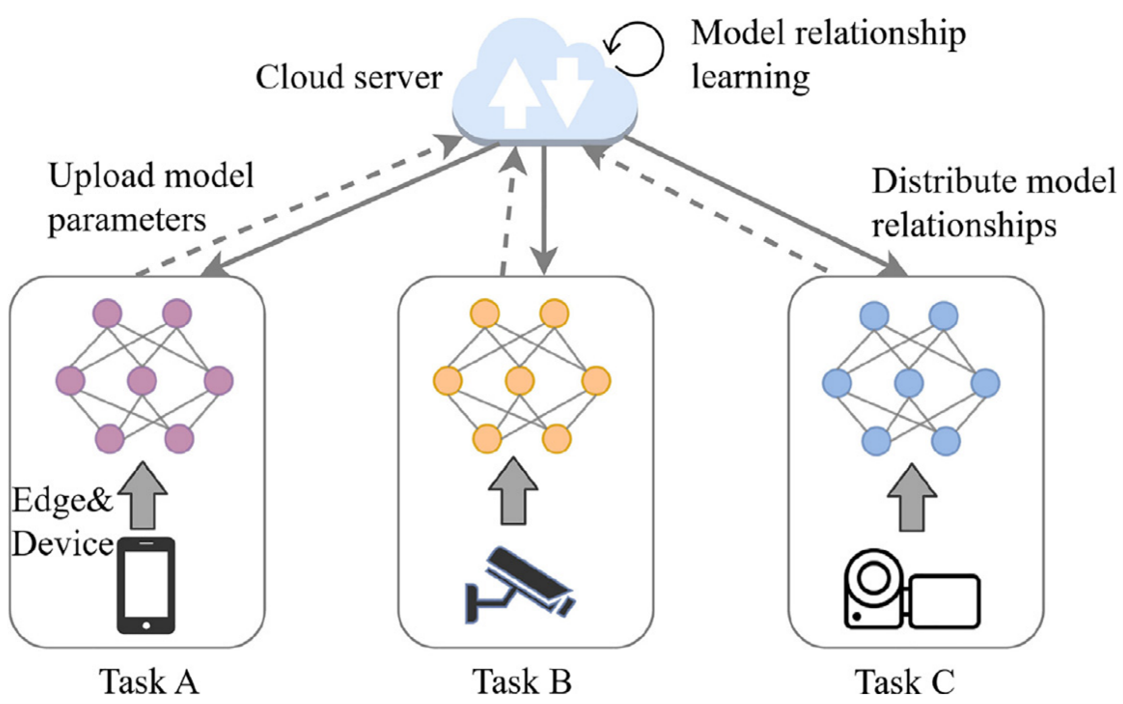
\includegraphics[scale=0.9]{images/chap3/multi_tasking.png}%
	\caption{%
		یادگیری فدرال چندوظیفه‌ای
		\cite{ma2022state}%
		.
	}
	\label{multi_tasking}
	\centering
\end{figure}


\subsection{
	یادگیری مادام‌العمر%
\LTRfootnote{Life-Long Learning}
}
رویکرد اصلی یادگیری مادام‌العمر به این صورت است که تلاش می‌کند در هر مرحله از الگوریتم، کاربرانی که برای اجرا انتخاب می‌شوند را به خاطر بسپارد. همان‌طور که پیش‌تر مطرح شد، در یادگیری فدرال ممکن است در هر مرحله تعداد کمی از کاربران انتخاب شوند. این مسئله باعث می‌شود که وزن‌ها و مدل‌هایی که برای کاربران جدید ارسال می‌شوند، لزوماً کارایی لازم را نداشته باشند. الگوریتم یادگیری مادام‌العمر تلاش دارد تا کاربران را به‌خاطر بسپارد و مدل‌های متناسب با هر کدام را ایجاد و به سمت آن‌ها ارسال کند
\cite{shoham2019overcoming}.

این رویکرد به این صورت عمل می‌کند که در هر مرحله از یادگیری، سوابق کاربران انتخاب شده را ذخیره می‌کند و از این سوابق برای بهبود و تطبیق مدل‌های آینده استفاده می‌کند. به این ترتیب، زمانی که کاربر جدیدی وارد فرآیند یادگیری می‌شود، الگوریتم می‌تواند از اطلاعات ذخیره شده قبلی استفاده کند و مدل بهتری را برای او ارسال کند. این روش باعث می‌شود که مدل‌ها به مرور زمان بهینه‌تر شده و عملکرد بهتری داشته باشند.

یکی از نکات مهم در یادگیری مادام‌العمر، حفظ و به‌خاطر سپاری کاربران است. در زمینه یادگیری فدرال، این کار به دلیل تعداد بسیار زیاد کاربران ممکن است چالش‌برانگیز باشد. یادگیری فدرال به‌طور معمول با تعداد زیادی از کاربران سروکار دارد و حفظ سوابق همه این کاربران به‌طور همزمان می‌تواند منابع زیادی را مصرف کند و پیچیدگی‌های فنی زیادی را به همراه داشته باشد.

در نتیجه، یادگیری مادام‌العمر با ذخیره و استفاده از اطلاعات کاربران در طول زمان، می‌تواند به طور مؤثری به مدیریت چالش‌های مربوط به داده‌های غیرمستقل و غیریکنواخت در یادگیری فدرال کمک کند و همچنین به حفظ و بهبود کارایی مدل‌های یادگیری فدرال کمک نماید.




